%                                                                 aa.dem
% AA vers. 8.2, LaTeX class for Astronomy & Astrophysics
% demonstration file
%                                                       (c) EDP Sciences
%-----------------------------------------------------------------------
%
%\documentclass[referee]{aa} % for a referee version
%\documentclass[onecolumn]{aa} % for a paper on 1 column  
%\documentclass[longauth]{aa} % for the long lists of affiliations 
%\documentclass[rnote]{aa} % for the research notes
%\documentclass[letter]{aa} % for the letters 
%\documentclass[bibyear]{aa} % if the references are not structured 
% according to the author-year natbib style

%
%\documentclass[twocolumn]{aastex61}

\documentclass[%
 aip,
 twocolumn,
 jmp,%
 amsmath,amssymb,
%preprint,%
 reprint,%
%author-year,%
%author-numerical,%
]{aastex61}
\usepackage{amsmath}
\usepackage{graphicx}% Include figure files
\usepackage{dcolumn}% Align table columns on decimal point
\usepackage{bm}% bold math
%\usepackage{aastex}

%\usepackage[mathlines]{lineno}% Enable numbering of text and display math
%\linenumbers\relax % Commence numbering lines
\newcommand{\Msun}{$M_{\odot}$}
\begin{document}

%\preprint{AIP/123-QED}

\title[MEASURING DARK MATTER PROFILES NON-PARAMETRICALLY IN DWARF SPHEROIDALS]{MEASURING DARK MATTER PROFILES NON-PARAMETRICALLY IN DWARF SPHEROIDALS:
	AN APPLICATION TO LEO I}% Force line breaks with \\
\thanks{Footnote to title of article.}


\date{\today}% It is always \today, today,
             %  but any date may be explicitly specified




\section{THE PROBLEM OF UNRESOLVED CROWDING}



The unresolved flux contribution by $j$ fainter stars to one given spectrum $i$, 
whose individual velocities $v_{ij}$ are randomly distributed around some mean value $\bar{v}$, will have the effect of biasing the measured velocity of 
such added spectrum $v_i$ towards $\bar{v}$.

If such resulting spectrum is to be confused with that 
of an individual star due to unresolved crowding, the effective 
standard deviation $\sigma$ of the measured velocities $v_i$ will be lowered
with respect to that of the actual stellar velocities $v_{ij}$
(just as the standard deviation of the mean of samples is smaller 
than the standard deviation of the entire sample).

\begin{figure}
\centering
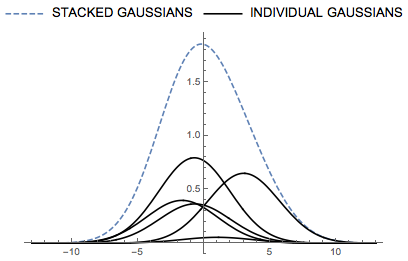
\includegraphics[width=0.5\textwidth]{CROWDING/UNRESOLVED_CROWDING.png}
\caption{UNRESOLVED CROWDING Ilustrated: The contribution from many gaussians appears as one gaussian centered closer to their mean when the gaussian width is close to the deviation of their centers.}       
\end{figure}

Particularly dense and faint environments are good candidates for this confusion.

In this section, we investigate the effects of unresolved crowding on the measurements of radial velocities for individual fibers on LEO I's most central regions.  We use two sets of deep, high resolution {\it Hubble Space Telescope (HST)} imaging to quantify the 
number of stars and their relative flux contribution to each fiber. The 
first set includes F435W imaging from the Advanced Camera for Surveys taken on 
February 2006 with an exposure time of 6800s (GO-10520; PI: Smecker Hane).
The second set includes F555W imaging from the Wide Field Camera 3 taken 
on January 2011 with an exposure time of 880s (GO-12304; PI: Holtzman).  
We create catalogs from both sets of imaging using daophot (REFERENCE).

Within our $3.2"$ diameter fibers we find a median of 20 stars in our deep
{\it HST} catalogs.  The brightest star in each fiber has a median
contribution of $30\%$ of the total flux. 

\begin{figure}
\centering
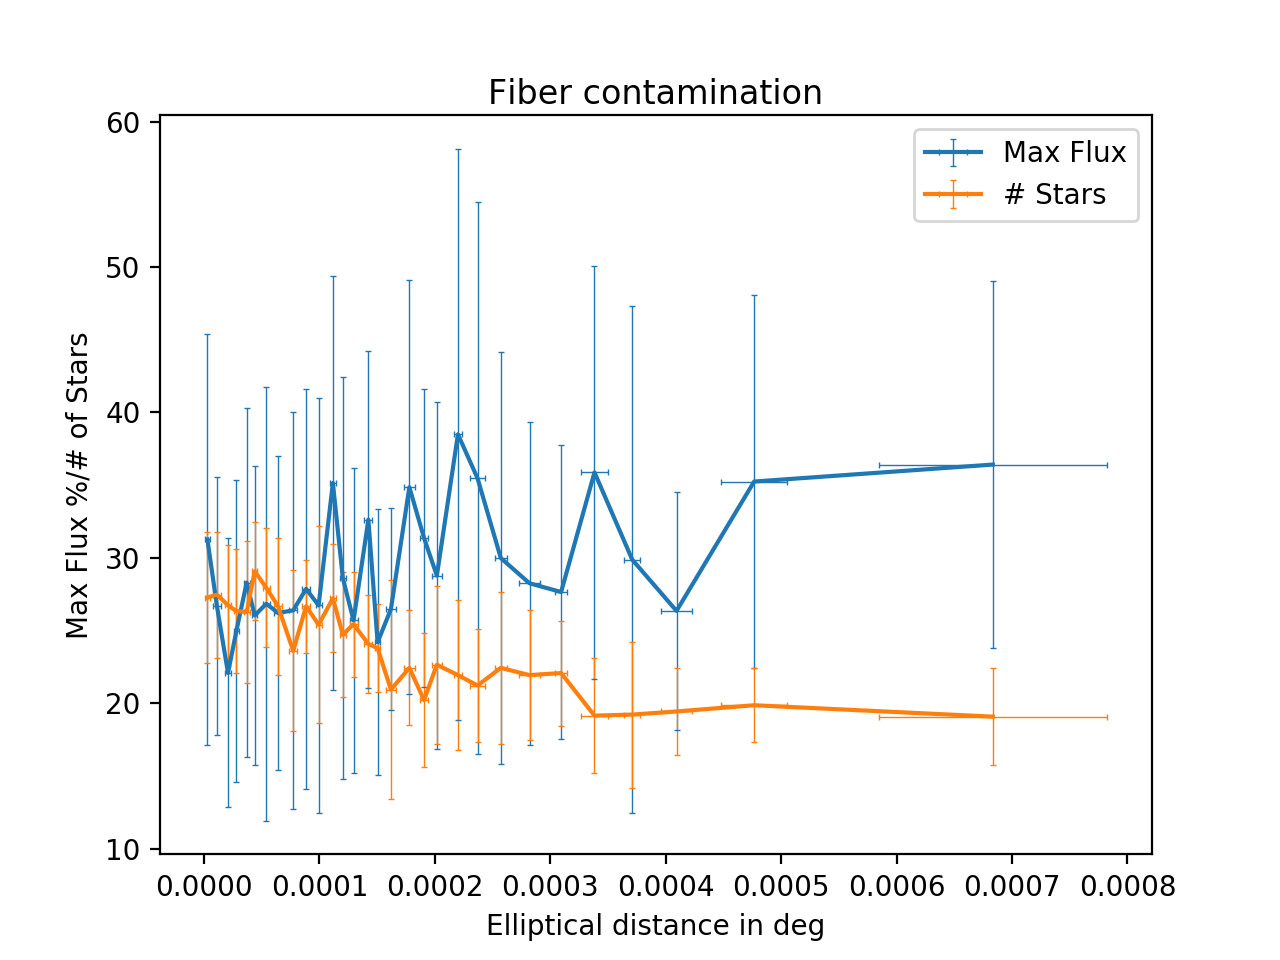
\includegraphics[width=0.5\textwidth]{CROWDING/fibercontamination.png}
\caption{Leo I data set using the deeper catalog, M08 fibers are excluded.}       
\end{figure}

Thus, no single star dominates the 
light of our fibers and rather we are capturing the light from small 
populations on the order of tens of stars each offset by their own individual
radial velocity. 
%On average, unresolved crowding on this scale biases the 
%radial velocity measurement of the fiber towards the systematic velocity of the
%system via the central limit theorem.  If the individual fiber radial velocities
%were used to measure the velocity dispersion, there would be a bias towards %lower
%dispersion measurements.  

In light of this unresolved crowding issue, we choose not
to measure radial velocities from individual VIRUS-W fibers but rather stack fibers
within radial bins and infer the velocity dispersion from the profiles of the
Mg b triplet absorption features.  Our kinematic measurements are discussed 
in more detail in \S X.

We also use an archival dataset from M08.  This program was able to target
individual, bright RGB stars which dominated the light in their fiber with 
some exceptions.  In the central 150 parsecs of Leo I, our {\it HST} catalogs
show that the HECTOCHELLE fibers captured the light from a median of X stars 
not including the central RGB target with a median contribution of $Y\%$ 
from the unresolved population.


\begin{figure}
\centering
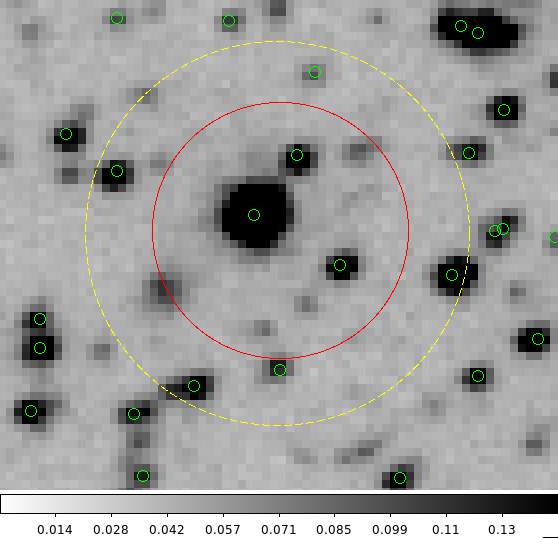
\includegraphics[width=0.5\textwidth]{CROWDING/FIBER_CROWDING.png}
\caption{M08 fiber # with catalogued stars overlaid. The red circle is the area covered by an HECTOCHELLE fiber (0.75" radius), the yellow stripped circle includes a bigger radius (+0.5") taken into account due to average seeing and pointing error for the observatory.}       
\end{figure}


Motivated to understand the effect this
might have on the kinematic measurements of M08 in the central 
regions of Leo I, we devise a simple model:

\begin{enumerate}
	\item We map the position of each contributing star 
	in relation to the fiber and derive their relative contribution 
	to the flux within that fiber based on distance to the center, seeing 
	conditions, and magnitude of the star. 
	
	\begin{equation}
	F(M_j,\mu_x,\mu_y) = A \,10^{-0.4 \times M}\int_{0}^{r} 
	e^{-\frac{(x-\mu_x)^2+(y-\mu_y)^2}{2\sigma^2}}dxdy
	\end{equation}
	
	Where $\sigma$ is the seeing/2.35, ($\mu_x$, $\mu_y$) are 
	the coordinates of the star with respect to the fiber center,
	$r$ is the radius of the fiber, $M$ is the star's apparent magnitude,
	and $A$ is a normalization constant.
	%This equation can be shown to further simplify to:	
	%\begin{equation}
	%F(M,c_d) = B \,10^M \int_{0}^{f_r}r  e^{-\frac{c_d^2+r^2}{2 \sigma ^2}} I_0\left(\frac{r c_d }{\sigma ^2}\right)dr
	%\end{equation}	
	%Which is now expressed just in terms of the star's distance to the fiber center $c_d$ (B again is some normalization constant). Considering we only need the relative flux contribution of the group of stars that fall within the fiber, we leave the overall normalization undefined. Hence, the relative flux contribution of \textbf{all} the stars on that fiber $\bar{F}$ is established.
	
	\item The absorption features in the spectra of the j$^{th}$ star 
	in the fiber are modeled with a Gaussian of width $\sigma_w$ 
	informed by that of the absorption lines of a template star. 
	
	\begin{equation}
	g_j(x) =  F_j \frac{\mathlarger{
	                    \mathlarger{e^{-\frac{(x-v_j)^2}
	                                         {2 \sigma_w ^2}
	                                  }
	                               }
	                    }}
	                   {\sqrt{2\pi}\sigma_w}
	\end{equation}
	
	\item $v_j(\sigma)$, the position of the $j$th gaussian in spectral space (the $j$th star's velocity) is randomly drawn from a normal distribution whose standard deviation (i.e., its velocity dispersion) is selected from range of 0.5 km/s to 60 km/s.
	\begin{align*}
	P(v_j,\sigma) = N(0,\sigma) \\
	\sigma \in [0.5,60]
	\end{align*}
	
	\item For each of the fibers, the gaussians are scaled to their relative flux contribution $F_j$ computed above and stacked in spectral space. 
	\begin{equation}
	G(x|\sigma) = \sum_{j \in \text{stars}}{g_j(x)}
	\end{equation}
	where we explicitly denote the random variable nature of the dependence on $\sigma$ to avoid confusion.
	\item The stacked gaussians are then cross-correlated with a
	normalized gaussian of width $\sigma_w$ to calculate the radial velocity $v_m$.
	\begin{equation}
    \arg\max( G(x|\sigma) \star
                          \frac{\mathlarger{
	                            \mathlarger{e^{-\frac{x^2}
	                                                 {2 \sigma_w ^2}
	                                          }
	                                       }
	                                       }
	                           }
	                   {\sqrt{2\pi}\sigma_w} 
	       ) = v_m
    \end{equation}
	\item We repeat this procedure 10,000 times for each
	input velocity dispersion to get the output velocity 
	distribution as well as the output velocity dispersion.
	This provides a map from input velocity dispersion to output
	velocity dispersion for a given flux distribution of contributing stars. This map, $\sigma_i(\bar{F}_i,\sigma)$,
	is produced for each $i$th fiber in M08 with {\it HST} imaging.

\end{enumerate}

\begin{figure}
\centering
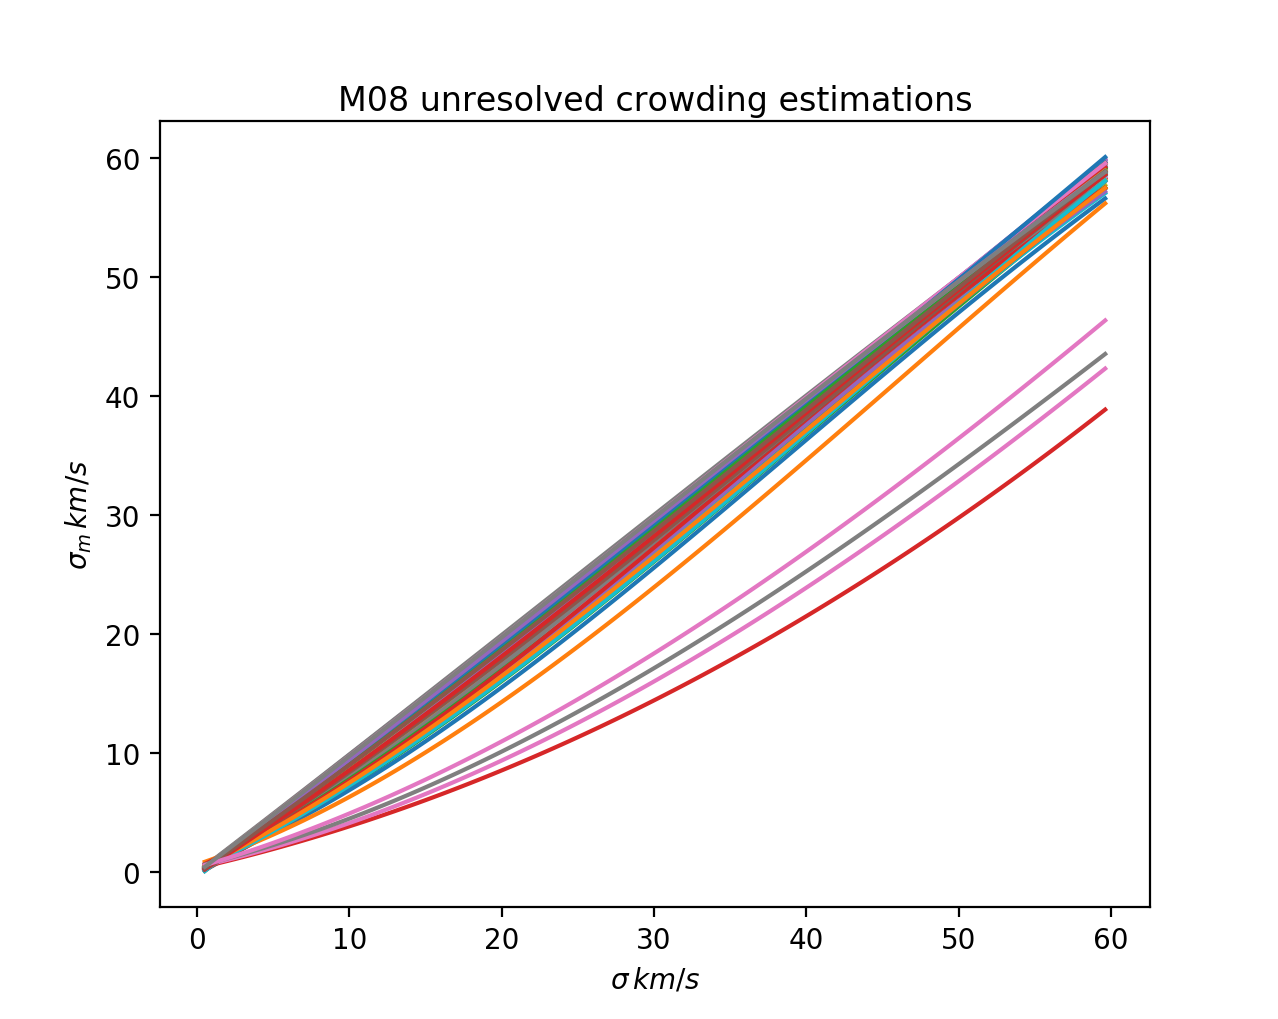
\includegraphics[width=0.5\textwidth]{CROWDING/M08FIBERMOD.png}
\caption{$\sigma_i(\bar{F}_i,\sigma)$ maps for M08 all fibers with HST coverage.}       
\end{figure}

Using this simple model and mapping allows us to construct a maximum likelihood
estimator (MLE) for the velocity dispersion of individual radial velocity measurements
from fibers in M08 with unresolved crowding issues.  The construction of such an MLE
is only applicable to the fibers with {\it HST} coverage, so 
we restrict our calculations and adjustments to fibers listed in table 1 in the appendix 
which satisfy this criteria. The difference between the shallow and deep {\it HST} catalogs 
is illustrated in fig ??. Whenever lacking deep imaging we resorted to the shallow catalog.
This will only have the effect of making our corrections less strong.
\begin{figure}
\centering
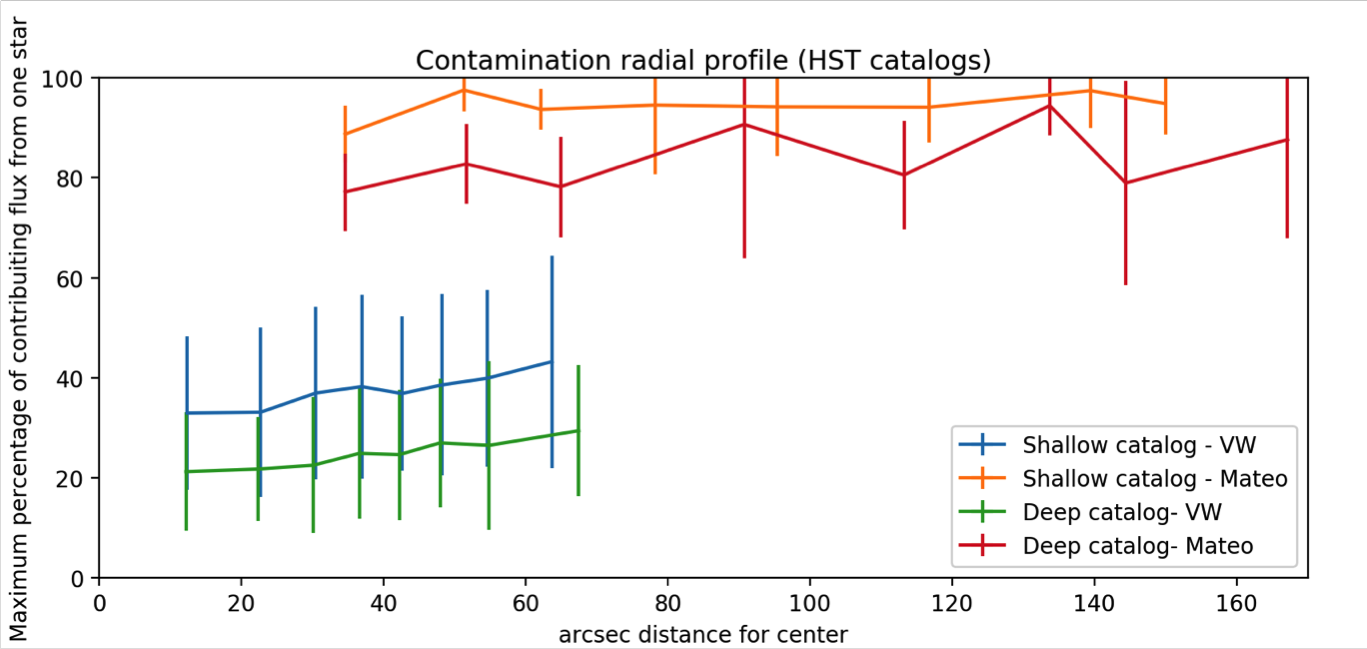
\includegraphics[width=0.5\textwidth]{CROWDING/RADIAL_CONTAMINATION.png}
\caption{Difference on maximum flux percentage from one star for both datasets and catalogs. Even
within {\it HST} catalogs the difference can be slightly larger than 10\%}       
\end{figure}
\begin{figure}
\centering
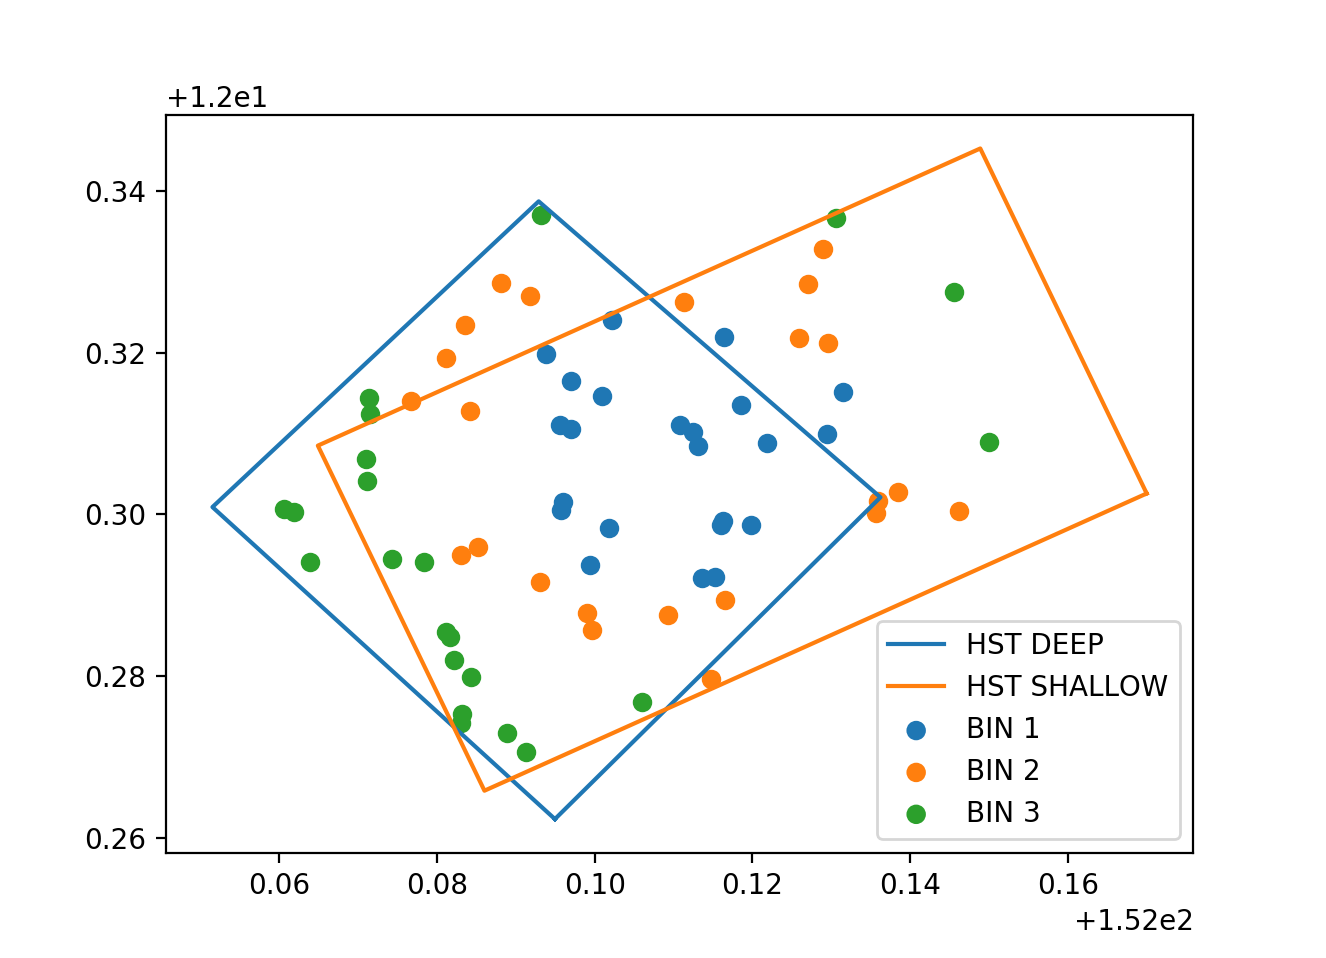
\includegraphics[width=0.5\textwidth]{CROWDING/CROWDING_HSTCOVERAGE.png}
\caption{Color coded bins within M08 with \it{HST} coverage.}       
\end{figure}

\begin{figure}
\centering
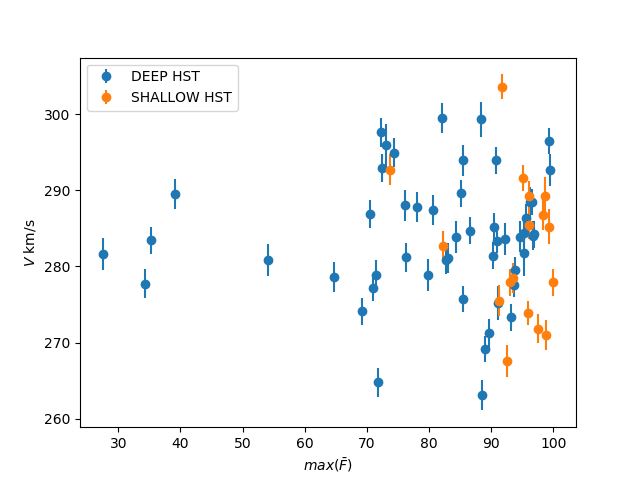
\includegraphics[width=0.5\textwidth]{CROWDING/VELvsCROWDING_MATEO.png}
\caption{M08 fibers arranged in terms of maximum flux from one star within a fiber. One can see a noticeable trend towards less dispersion depending on flux percentage.}       
\end{figure}


%\begin{multline*}
%P(v_i|\bar{M_{i}},\sigma,h_3,h_4)=\\
%\frac{e^{-\frac{(y-\mu)^2}{2 \sigma %_i^2}}}{\sqrt{2 \pi } \sigma _i}
%\otimes
%\frac{\left(e^{-\frac{(y-\mu )^2}{2 \sigma _p^2}} 
%\left(
%	1+
%	h_3\frac{ H_3 (\frac{y-\mu}{\sigma _p})}{\sqrt{2^3 3!} }+
%    h_4\frac{ H_4 (\frac{y-\mu}{\sigma _p})}{\sqrt{2^4 4!} }
%\right)\right)}
%{\sqrt{2 \pi } \sigma _p }
%\end{multline*}

For a given radial bin, we calculate the probability of measuring a particular velocity $v_{m_i}$,

\begin{align}
P(v_{m_i}|\sigma_i,\sigma_e)=
\mathlarger{\mathlarger{\frac{e^{-\frac{(v_{m_i}-\mu)^2}{2 \sigma_e^2}}}{\sqrt{2 \pi }\sigma_e} \otimes
                        \frac{e^{-\frac{(v_{m_i}-\mu)^2}{2 \sigma_i^2}}}{\sqrt{2 \pi }\sigma_i}}}
\end{align}

Where $\otimes$ denotes convolution,

\begin{align*}
\mu = \mu(\sigma_i,\sigma_e) &= 
\mathlarger{
\mathlarger{
\frac{\sum_i \frac{v_{m_i}}{\sigma_i^2+\sigma_e^2}}
     {\sum_i \frac{1}    {\sigma_i^2+\sigma_e^2}}
}},
\end{align*}
and
\begin{align*}
\sigma_i &= \sigma_i(\bar{F}_i,\sigma).
\end{align*}
The mapping, $\sigma_i$, is from our simple model above,
the index i represents the i$^{th}$ fiber in the bin,
$\bar{F}_i$ is the flux vector of stars in the ith fiber,
$\sigma_e$ is the radial velocity measurement error, and
$\sigma$ is the velocity dispersion in the bin without any
crowding correction.

Thus, we maximize the likelihood ${\mathcal{L(\sigma)}}$ for a given bin to get our best estimate of the true velocity dispersion
\begin{align*}
\mathcal{L(\sigma)} = \prod^N_iP\left(v_{m_i}|\sigma_i,\sigma_e\right)\\
\sigma = \arg\max\mathcal{L(\sigma)}
\end{align*}

Our correction to the most inner M08 bins are shown in figure ??. 
\begin{figure}
\centering
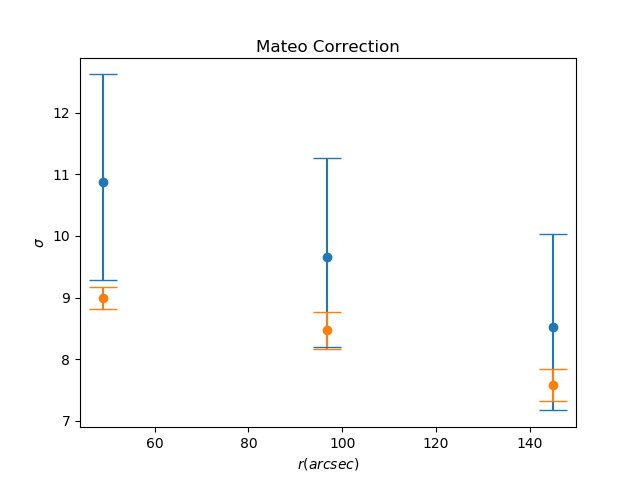
\includegraphics[width=0.5\textwidth]{CROWDING/mateo_corrections.png}
\caption{Bin corrections for M08 fibers within \it{HST}.}       
\end{figure}

Even though the coverage is not complete, one can extrapolate the results to the other
fibers making use of the surface density profile as shown in figure ??.


\end{document}


